\section{Comparison with other methods in terms of performance} \label{comparison}

In this section we aim to give a quantitative comparison on standard object detection datasets of the YOLO method and the methods described in Section \ref{related_work}. 

To measure an object detection system performance usually frames per second (FPS) and mean average precision (mAP) are the most relevant measures. FPS simply means the number of images, or frames, an algorithm can process in a single second.

%In order to see how accurate the model is, mAP is used. To compute mAP, first, the predictions are sorted descending by their confidence score. Then, the predictions are parsed one by one, and at each step, the precision and recall are computed, taking into consideration only the parsed prediction up until that point. For the recall, we consider all positives, including those that were not parsed. If we would plot these values, with the recall on the horizontal axis and the precision on the vertical axis, we would get what is called the precision-recall curve. Average precision is defined as the area under the precision-recall curve and mAP is defined as the mean of the average precisions for each class.

Over time, this mAP measure became the standard when it comes to measuring the quality of an object detection system.

The first standard dataset in object detection research was The Pascal Visual Object Classes \cite{pascal-voc} and it started out as an object detection challenge. Basically, the researchers that came up with new ideas in this domain had to use this dataset in order to compare their methods with the existing literature. Additionally, in order for the comparison to be fair, the authors of the dataset also published the code for computing mAP.

In Fig. \ref{pascal} we detail the mAP values for some object detectors described early. We can see that the original YOLO methodology lags behind other object detectors, but the second one, which introduces anchors, surpasses them all.


\def \scalevar {0.6}

\begin{figure}[!h]
  \centering
  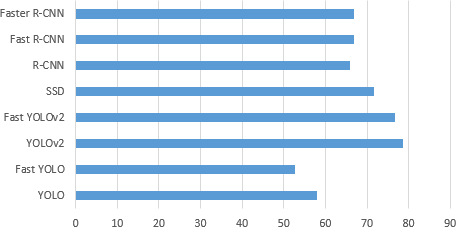
\includegraphics[scale=\scalevar]{images/pascal.png}
  \caption{Performances over the Pascal VOC dataset in terms of mAP}
  \label{pascal}
\end{figure}

As the technology advanced, researchers were able to train on larger and larger datasets, thus the Microsoft Common Objects in Context (COCO) dataset \cite{coco} became the new standard that new object detection methodologies use in order to be relevant in the field. Also, the authors provide an evaluation server which allows a better comparison between object detectors. The idea is that the labels for the test set are not publicly available, only the images can be downloaded. Therefore, the researchers that propose new object detection methods, have to upload on the evaluation server their results on the test set, and get back a detailed mAP evaluation for various thresholds and for small, medium and large objects.

We also perform a comparison on the newer standard COCO dataset in Fig. \ref{coco}. Here we can observe that YOLO had a constant positive evolution through time on this dataset.

\begin{figure}[!h]
  \centering
  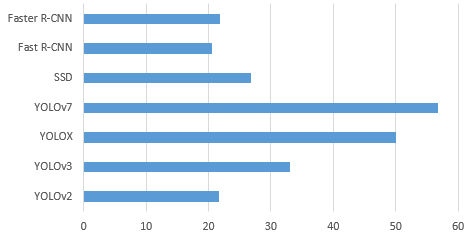
\includegraphics[scale=\scalevar]{images/coco.png}
  \caption{Performances over the COCO dataset in terms of mAP}
  \label{coco}
\end{figure}


Also, another crucial aspect is the speed. In Fig. \ref{fps} we detail the reported speeds in FPS. This measure is relevant in practical applications, because usually, the hardware is a pretty rigid constraint, and as such the neural network that runs on the hardware must meet the some speed constraints in order to run as expected from the point of view of the application. For example, R-CNN like methods are better suited for applications where real time speed is not crucial, and the others are built specifically for real time speeds.

\begin{figure}[!h]
  \centering
  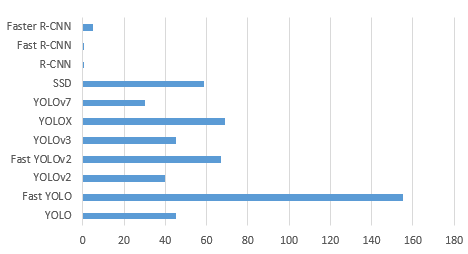
\includegraphics[scale=\scalevar]{images/speed.png}
  \caption{Performances in terms of frames per second}
  \label{fps}
\end{figure}





%Regarding performance on the Pascal VOC 2007 dataset, SSD achieves 74.3\% mAP and 59 FPS, surpassing the first version of YOLO in terms of speed and accuracy balance.
        
%On the Microsoft COCO and in the context in which YOLOv4 was tested, described in \cite{yolov4}, SSD achieves 43 FPS with 25.1\% mAP. This shows that YOLO surpasses SSD in terms of prediction quality, with minimal time costs.


%According to \cite{yolo}, in terms of performance on the Pascal VOC 2007 dataset \cite{pascal-voc-2007}, the first version of YOLO achieves 63.4\% mAP and 45 frames per second (FPS), and the faster version has 52.7\% mAP and 155 FPS. For comparison, Faster R-CNN \cite{fasterRcnn} achieves 73.2\% mAP but 7 FPS, which is accurate but very slow, and the Deformable parts model \cite{30hzDPM} achieves 100 FPS but it has 16\% mAP, or a slower variant achieves 26.1\% mAP at 30 FPS. Therefore YOLO strikes a good balance between speed and accuracy.
    
%Newer versions of YOLO bring some incremental improvements. Also, the Microsoft COCO dataset \cite{coco} is another relevant dataset for comparing object detection systems. On this dataset, YOLOv4 \cite{yolov4} achieves 43.9\% mAP at 31 FPS, or a smaller variant achieves 38 FPS, with 41.2\% mAP.

